\begin{frame}[Core Problem ]
\frametitle{Core Problem Statement}
\begin{itemize}
\item Refer Petrini et al for early work on ASCI Q.
\item Refer Hoefler  et al for up-to-date work  (clearly identifies ``resonance'' issue as number of processors are increased). 
\end{itemize}
\end{frame}

\begin{frame}[Traditional Data Parallelism]
\frametitle{Core Problem Statement}
\begin{itemize}
\item We can take advantage of the parallelization by trying to do a
  perfect domain decomposition and splitting work evenly across
  threads. 
\item The assumption here is that all the processing elements will be used all the time. 
\end{itemize}
\end{frame}

\begin{frame}[MPI domain decomp]
\frametitle{Standard MPI domain decomposition}
  \begin{figure}
    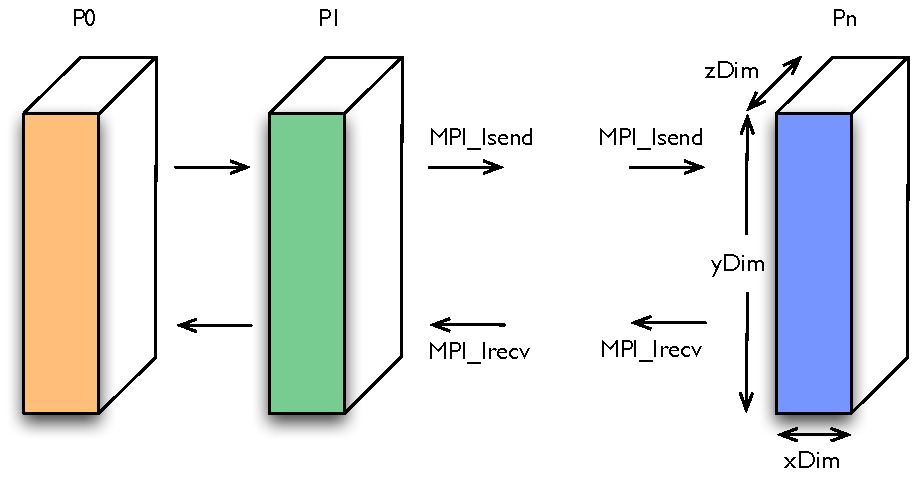
\includegraphics[width=0.65\textwidth]{images/mpi_decomp}
  \end{figure}
\end{frame}

\begin{frame}[Domain Decomp with uSched]
\frametitle{MPI domain decomposition with lightweight scheduling incorporated}
  \begin{figure}
    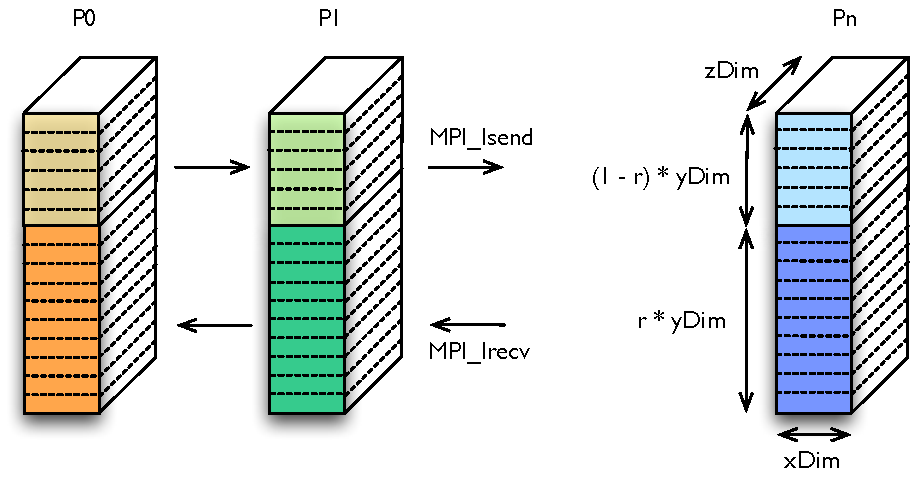
\includegraphics[width=0.65\textwidth]{images/hybrid_decomp}
\end{figure}
\end{frame}

\begin{frame}[Separate Solutions]
\frametitle{Separate Solutions}
  \begin{itemize}

  \item \textit{Application-level:} 
    \begin{itemize}
    \item using auto-tuned micro-scheduling
    \item abstractions for tuning micro-scheduling
    \end{itemize}

  \item \textit{Runtime-level:} 
    \begin{itemize}
    \item Can use online machine learning to assess performance variation and tune accordingly at runtime. 
    \item Could develop (or extend) an ``intelligent'' runtime system that automatically handles noise mitigation behind the scenes, detecting patterns in noise load imbalance through measurements taken at runtime. 
    \end{itemize}


  \item \textit{System-level:}
    \begin{itemize}
    \item co-scheduling and gang-scheduling 
    \item process migration
    \end{itemize}


  \item \textit{Platform-level:}
    \begin{itemize}
    \item judiciously stripping away OS services
    \item Creating abstractions to strip away such services
    \end{itemize}
  \end{itemize}
\end{frame}

